% !TEX program = xelatex
\documentclass[b5paper, 11pt, openleft]{memoir}

\usepackage{indentfirst}

%%% Font setup
\usepackage[no-math]{fontspec}
\setmainfont{Zilla Slab}
\setmonofont[Scale = MatchLowercase]{Iosevka Custom Medium Condensed}
\XeTeXlinebreaklocale="en_EN"
\XeTeXlinebreakskip=0pt plus 3pt
\emergencystretch=1em

\usepackage{mathtools}
\usepackage[math-style = ISO, mathrm = sym, warnings-off = {mathtools-colon}]{unicode-math}
\setmathfont[Scale = MatchLowercase]{Concrete-Math.otf}
\noDisplayskipStretch
\setoperatorfont\symscr
\everymath{\displaystyle}

%%% Stylings
% Page Layout and Margins
\setsecnumdepth{subsection}
\settocdepth{subsection}
\setlrmarginsandblock{4cm}{1.5cm}{*}
\setulmarginsandblock{3cm}{2.5cm}{*}
\setlength{\headheight}{30pt}
\setlength{\parindent}{1.5cm}
\setlength{\parskip}{0.3em}
\setlength{\beforechapskip}{20pt}
\renewcommand{\arraystretch}{1}
\allowdisplaybreaks
\setSpacing{1.5}
\checkandfixthelayout

% Footnotes
\usepackage{fancyhdr}
\pagestyle{fancy}
\fancyhead[LE]{\textbf{\thepage ~ $\big\vert$ \leftmark}}
\fancyhead[RO]{\textbf{\rightmark ~ $\big\vert$ \thepage}}
\fancyhead[RE, LO, C]{}

% Styling Figures
\usepackage{multicol, caption}
\setlength{\columnseprule}{1pt}
\def\columnseprulecolor{\color{lightgray}}
\DeclareCaptionLabelSeparator{pipe}{ $\vert$ }
\captionsetup{
    labelfont = {bf},
    font = {small, sc},
    width = 0.6\textwidth,
    labelsep = pipe,
    figurename = \textbf{Fig. }
}

% Styling Titles
\renewcommand{\partnamefont}{\LARGE\bfseries\scshape\centering}
\renewcommand{\partnumfont}{\LARGE\bfseries\scshape\centering\MakeUppercase}
\renewcommand{\midpartskip}{\par\rule{1in}{0.5pt}\vspace{1em}\par}
\renewcommand{\printparttitle}{\HUGE\bfseries\scshape\centering}
\renewcommand{\afterpartskip}{\relax}
\chapterstyle{veelo}
    \renewcommand*{\printchapternum}{%
    \makebox[0pt][l]{%
    \hspace{.8em}%
    \resizebox{!}{\beforechapskip}%
    {\chapnumfont \thechapter}%
    \hspace{.8em}%
    \rule{2\midchapskip}{\beforechapskip}%
    }%
}

% Packages
\usepackage[dvipsnames]{xcolor}
\usepackage{subcaption, graphicx, pdfpages, float, wrapfig}
\usepackage{minted}
\usemintedstyle{base16-unikitty-light}
\setminted{
    frame = lines,
    bgcolor = lightgray!20,
    linenos,
	breaklines,
	fontsize = \small
}
\usepackage{csquotes}
\graphicspath{{figures/}}
\usepackage[inline]{enumitem}

\usepackage[colorlinks, allcolors = blue]{hyperref}
\usepackage{cleveref}

%%% Mathematical packages 
\usepackage[]{siunitx}
\usepackage{physics2}
\usepackage{derivative}
\usephysicsmodule{ab, ab.braket, nabla.legacy, op.legacy}
\usephysicsmodule{ab.legacy}
\usepackage[makeroom]{cancel}
% Proofs
\usepackage{amsthm}
\usepackage{tcolorbox}
\tcbuselibrary{breakable, theorems, skins}
\newtcbtheorem[auto counter, crefname = {theorem}{theorems}, Crefname = {Theorem}{Theorems}]{theorem}{Theorem}{
    coltitle = black,
    sharp corners, frame hidden, enhanced, colback = lightgray!10, breakable,
    borderline west = {3pt}{-3pt}{lightgray},
    detach title = true,
    fonttitle = \bfseries, before upper = {\tcbtitle\quad}
}{theorem}
\newtcbtheorem[auto counter, crefname = {axiom}{axioms}, Crefname = {Axiom}{Axioms}]{axiom}{Axiom}{
    sharp corners, colback = lightgray!40, colframe = darkgray, breakable
}{axiom}
\newtcbtheorem[auto counter, crefname = {definition}{definition}, Crefname = {Definition}{Definition}]{df}{Definition}{
    sharp corners, colback = lightgray!40, colframe = darkgray, breakable
}{df}
\newtcbtheorem[auto counter, number within = section]{exmp}{Example}{
    colback = lightgray!40, colframe = darkgray, breakable
}{exmp}
\newtcbtheorem[auto counter, number within = chapter, crefname = {remarks of chapter }{remarks of chapter }, Crefname = {Remarks}{Remarks}]{remark}{Remarks on chapter }{
    colback = lightgray!10, colframe = black, breakable
}{remark}

%%% Mathematical commands
% Geometry
\let\line\overline
% Mathematical constants
\newcommand{\e}{\symrm{e}}
\newcommand{\im}{\symrm{i}}
\newcommand{\cpi}{\symrm{\pi}}
\DeclareMathOperator*{\ssum}{\symrm{\Sigma}}
\DeclareMathOperator*{\Proj}{\symrm{Proj}}
\DeclareMathOperator*{\sgn}{\symrm{sgn}}
% Vector notations
\newcommand{\vv}[1]{\pmb{\symrm{#1}}}
\newcommand{\vdot}{\pmb{\cdot}}
\newcommand{\conj}{^{\ast}}
\newcommand{\dagr}{^{\dag}}
\newcommand{\trnsp}{^{\intercal}}
\newcommand{\iden}{\symbb{I}}
\newcommand{\uv}[1]{\hat{\vv{e}}_{#1}}
\newcommand{\tensor}{\otimes}
\newcommand{\bmat}[1]{
	\begin{bmatrix}
		#1
	\end{bmatrix}
}
\newcommand{\ihat}{\hat{\i}}
\newcommand{\jhat}{\hat{\j}}
\newcommand{\khat}{\hat{k}}
\newcommand{\xhat}{\hat{\vv{x}}}
\newcommand{\yhat}{\hat{\vv{y}}}
\newcommand{\zhat}{\hat{\vv{z}}}
\newcommand{\rhat}{\hat{\vv{r}}}
\newcommand{\nhat}{\hat{\vv{n}}}
\newcommand{\that}{\hat{\vv{\theta}}}
\newcommand{\phat}{\hat{\vv{\rho}}}
\newcommand{\eflux}{\symrm{\Phi}_E}
\newcommand{\mflux}{\symrm{\Phi}_B}
\newcommand{\sint}{\int_{\mathcal{S}}}
\newcommand{\aint}{\int_{\mathcal{A}}}
\newcommand{\vint}{\int_{\mathcal{V}}}
\newcommand{\cint}{\int_{\mathcal{C}}}
\newcommand{\bperm}{\symrm{\mu}_0}
\newcommand{\eperm}{\symrm{\varepsilon}_0}
\newcommand{\rc}{{{\mbox{$\resizebox{1.2ex}{1.15ex}{\includegraphics[trim= 1em 0 14em 0,clip]{fonts/scriptr.pdf}}$}}}}
\newcommand{\brc}{{{\mbox{$\resizebox{1.2ex}{1.15ex}{\includegraphics[trim= 1em 0 14em 0,clip]{fonts/boldcursiver.pdf}}$}}}}
\newcommand{\rchat}{{{\mbox{$\hat\rcurs$}}}}
\newcommand{\peval}[1]{\left(\left.#1\right.\right\rvert}
% Differences
\DeclareMathOperator{\kdel}{\symrm{\delta}}
\DeclareMathOperator{\ddel}{\symrm{\delta}}
\newcommand{\Dd}{\symrm{\Delta}}
% Physics quantities symbols
\newcommand{\lagr}{\mathcal{L}}
\newcommand{\haml}{\mathcal{H}}
\newcommand{\hilb}{\mathcal{E}}
\newcommand{\emf}{\mathcal{E}}
% Calculus notations
\newcommand{\appr}{\rightarrow}
\newcommand{\alc}[2][0.3]{&\parbox[c]{#1\textwidth}{#2}}
\newcommand{\pintm}[1]{\mathcal{D}[#1]}
% Mathematical conjunctions and expressions
\newcommand{\mathand}{\quad\textrm{and,}\quad}
\newcommand{\mathor}{\quad\textrm{or,}\quad}
\newcommand{\mathif}{\quad\textrm{if}\quad}
\newcommand{\mathiff}{\quad\textrm{\emph{iff}}\quad}
\newcommand{\maththerefore}{\therefore\emquad}
\newcommand{\ifft}{\emph{iff}}
% Notational commands
\newcommand{\flatfrac}[2]{#1\fracslash#2}
% Column types
\newcolumntype{C}{>{$}c<{$}}
\newcolumntype{L}{>{$}l<{$}}
\newcolumntype{R}{>{$}r<{$}}

%%% Type commands
\newcommand{\conclusion}{\section{Conclusion for Chapter \thechapter}}
\newcommand{\formula}{\section{Formula from Chapter \thechapter}}
\newcommand{\prelude}[1]{
    \chapter*{Prelude: #1}
    \addcontentsline{toc}{chapter}{Prelude: #1}
}
\newcommand{\prerequisites}[1]{\textbf{Prerequisites:}~\emph{#1}}

% Bibliographies
\usepackage[
    backend = biber,
    style = phys,
    sorting = anyvt
]{biblatex}
\addbibresource{bibfile.bib}

\usepackage[inkscapeversion = 1, inkscapelatex = true]{svg}
\svgpath{{code/}}
% Indices
\usepackage{imakeidx}
\makeindex

\begin{document}

\frontmatter
\title{
	\vspace{-5em}
	\textbf{
		AI Builders: 2D Fluid simulation framework via the Lattice-Boltzmann method with conditional optimizers
	}
}
\author{
	Puripat Thumbanthu, Kunakorn Chaiyara \\
	Documentation written by Puripat Thumbanthu
}
\date{Started: November 11, 2024; Revision: \today}
\maketitle

\tableofcontents*

\mainmatter

\chapter{Introduction}

\section{Backgrounds}

This project, submitted to the \texttt{AI Builders X ESCK} program, originated from a series of questions.
\begin{itemize}
	\item What's the best way to blow on a liquid filled spoon to cool it?
	\item Given a room, what's the best place to place an air conditioner, and what direction must it face?
	\item What's the best place for a cooling fan in a CPU?,
\end{itemize}
etc. These problems are a set of problems that all fall in optimization problems in fluids:
\begin{quote}
	\emph{"Given an imposed boundary condition on a system containing fluids, a boundary condition that's free to move, and a certain function, find the boundary condition that optimizes the function."}
\end{quote}
E.g., in the first problem, the imposed boundary condition is the shape of the room; the free boundary condition is the placement and angle of the air conditioner, and the function is the time until the room reaches thermal equilibrium.

Due to the ten weeks time limit imposed by the \texttt{AI Builders X ESCK} program. We've decided to simplify various parts of the problem to make it more fathomable.

\section{Problem statement and overview of solution}

The problem that we've selected to tackle is the second problem due to phase homogeneity: \enquote{given a room, what's the best place to place an air conditioner, and what direction must it face.} Due to complexity in three-dimensions, we've decided to simplify the problem to a room with boundaries in two-dimensions, and only allow the air conditioner to exist on a line around the border of the room.

The variables that are used in this problem is as follows:
\begin{enumerate}[noitemsep]
	\item \textbf{The function needed for optimization}---the time until equilibrium
	\item \textbf{Free boundary condition}---placement of the air conditioner, represented as a density boundary condition
	\item \textbf{Imposed boundary condition}---shape of the room
\end{enumerate}
It's then solved as follows:
\begin{enumerate}[noitemsep]
	\item Build a fluid simulator with wall and density boundary condition,
	\item Input the shape of the room, and the strength of the air conditioner,
	\item Find the optimal air conditioner using gradient descent.
\end{enumerate}

Originally, we planned to use the \texttt{OpenFOAM} simulator, as it's commonly used by researchers in computational fluid dynamics. However, the learning curve is too steep for just ten weeks. There's no clean way to connect the data from \texttt{OpenFOAM} into \texttt{Python} for post-processing. Most importantly, there aren't many great resources out there. So, we've decided to build our own simulation and optimization algorithm from scratch using one of the most accessible methods to do fluid simulation: the Lattice-Boltzmann method.

\section{Overview of the Lattice-Boltzmann method}

The Lattice-Boltzmann method is a fluid simulation method that doesn't require discretization of the Navier-Stokes equation. Instead, it models fluids as a collection of particles in a lattice filled with cells. In each step of the simulation, the particle moves from its own cell to its adjacent cells. Then, it interacts inside the cell through self-collisions. This cell-interpretation allow the derivation of the macroscopic fluid properties, e.g., density and velocity, to be derived from the particle distributions in each lattice directly. The process includes
\begin{enumerate}
	\item \textbf{Streaming}---particles move into adjacent cells
	\item \textbf{Collisions}---the densities in each cell is adjusted towards equilibrium inside the cell.
\end{enumerate}

This method is very viable for parallel computing, making it very ideal for implementation in \texttt{NumPy}. However, it is numerically unstable for high-speed fluid flows near or above the speed of sound. Since we're not dealing with particles moving that fast, we should be fine.

Even though the Lattice-Boltzmann method is stable for the most part, it still has some numerical instabilities around boundary conditions especially anything to do with circles. These will become a problem in gradient descent, in which we have to implement an algorithm to work around these instabilities.

\subsection{Representation}

\paragraph{Coordinate convention} Since \texttt{NumPy} indexes the $y$-axis (vertically) before the $x$-axis (horizontally), all pairs of coordinates from now on is to be read as $(y, x)$, not $(x, y)$

A fluid simulation with resolution $N \times M$ illustrated in \cref{fig:fluid-lattice}, is represented as a rectangular lattice with $N \times M$ cells. Each cell in the lattice contains nine cell-invariant unit vectors, $\vv{e}_0$ to $\vv{e}_8$, which represents the eight possible direction that the fluid can travel in. The value for these vectors, respective to the Cartesian representation is given in \cref{tab:unit-vectors}

\begin{table}[ht]
	\centering
	\begin{tabular}{C | C}
		\textrm{Unit vector} & \textrm{Representation} \\
		\hline
		\vv{e}_0             & \vv{0}                  \\
		\vv{e}_1             & \xhat                   \\
		\vv{e}_2             & \yhat                   \\
		\vv{e}_3             & -\xhat                  \\
		\vv{e}_4             & -\yhat                  \\
		\vv{e}_5             & \xhat + \yhat           \\
		\vv{e}_6             & -\xhat + \yhat          \\
		\vv{e}_7             & -\xhat - \yhat          \\
		\vv{e}_8             & \xhat - \yhat
	\end{tabular}
	\caption{Unit vectors used in a cell of fluid}
	\label{tab:unit-vectors}
\end{table}

\begin{figure}[ht]
	\centering
	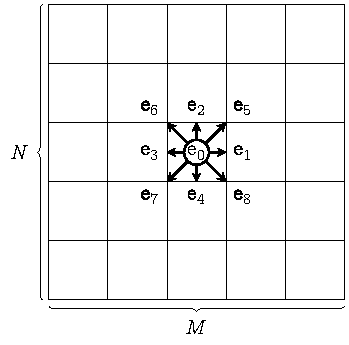
\includegraphics{fluid-lattice.pdf}
	\caption{Lattice of fluid}
	\label{fig:fluid-lattice}
\end{figure}

From the set of vectors $\vv{e}_0, \dots, \vv{e}_8$ inside each cell, one respectively assign another set of vectors $\vv{f}_0, \dots, \vv{f}_8$. These vectors are scaled version of the unit vectors, i.e.,
\begin{equation}
	\vv{f}_i = f_i\vv{e}_i,
\end{equation}
where the scalar $f_n$ represents the amount of fluid that's moving in the direction $\vv{e}_n$. From this representation alone, the density, momentum, and speed of the fluid at a certain point $(n, m)$ can be found. The density of fluid at the cell $(n, m)$, $\rho(n, m)$, is the sum from of all $f_i$'s inside the cell:
\begin{equation}
	\rho(n, m) \equiv \sum_if_i(n, m). \label{eq:density-calculation}
\end{equation}
The momentum density, $\vv{U}(n, m)$, traditionally given by the product between velocity and mass, can be calculated as the sum of product between $f_n$ and their respective unit vectors:
\begin{equation}
	\vv{U}(n, m) \equiv \sum_nf_n\vv{e}_n. \label{eq:momentum-calculation}
\end{equation}
The velocity density at a certain cell is just the ratio between the momentum density and the fluid density:
\begin{equation}
	\vv{u}(n, m) \equiv \frac{\vv{U}(n, m)}{\rho(n, m)} = \frac{\sum_nf_n\vv{e}_n}{\rho}. \label{eq:velocity-calculation}
\end{equation}

\subsection{Self-collision step}

The self-collision step represents the relaxation of fluid that happens inside a cell. In each of the fluid vectors $\vv{f}_0,\dots,\vv{f}_8$, a corresponding equilibrium vector is assigned by
\begin{equation}
	\vv{E}_i(n, m) = w_i\rho\ab(1 + 3\vv{e}_i \cdot \vv{u}(n, m) + \frac{9}{2}\ab(\vv{e}_i \cdot \vv{u}(n, m))^2 - \frac{3}{2}|\vv{u}(n, m)|^2)\vv{e}_i \label{eq:self-collision-calculation-1}
\end{equation}
where $w_i$ is a weighting factor that's given by the reduction of Boltzmann's distribution:
\begin{gather}
	w_i = \begin{cases}
		\frac{4}{9}  & \textrm{if} ~ i = 0,          \\
		\frac{1}{9}  & \textrm{if} ~ i = 1, 2, 3, 4, \\
		\frac{1}{36} & \textrm{if} ~ i = 5, 6, 7, 8.
	\end{cases}
\end{gather}
The corresponding equilibrium scalar $E_i(n, m)$, is given by the relation
\begin{equation}
	\vv{E}_i(n, m) = E_i(n, m)\vv{e}_i.
\end{equation}

However, a fluid cannot possibly reach its own equilibrium in just one step; therefore, the Lattice-Boltzmann adjusts the fluid vector to approach the equilibrium vector. This behavior is captured by the relaxation time $\tau$. For the set of fluid vector positioned at the cell $(n, m)$ at time $t$, $f_i(n, m; t)$, the fluid vector at the next time step, $t + \Dd{t}$ is given by
\begin{equation}
	f_i(n, m; t + \Dd{t}) = f_i(n, m; t) + \frac{1}{\tau}\ab(E_i(n, m; t) - f_i(n, m; t)), \label{eq:self-collision-calculation-2}
\end{equation}
and that
\begin{equation}
	\vv{f}_i(n, m; t + \Dd{t}) = f_i(n, m; t + \Dd{t})\vv{e}_i.
\end{equation}

The relaxation value that's used throughout this project is $\tau = 0.8070$, which is said to be the most numerically stable \cite{zhao-2013}.

\subsection{Streaming step}

Using the vector that's adjusted to the equilibrium from the self-collision step, that vector is streamed to the adjacent cells, given by
\begin{equation}
	\vv{f}_i\ab(n + (\yhat \vdot \vv{e}_i), m + (\xhat \vdot \vv{e}_i)) = \vv{f}_i(n, m; t + \Dd{t}).
\end{equation}
Basically, this equation moves the fluid from one cell to the other as illustrated in \cref{fig:streaming-step}
\begin{figure}
	\centering
	\begin{subfigure}{0.45\textwidth}
		\centering
		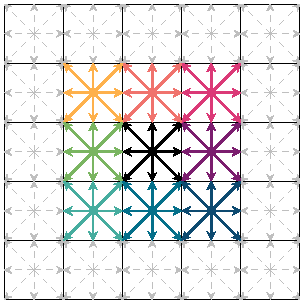
\includegraphics{streaming-before.pdf}
		\caption{Before}
	\end{subfigure}
	\begin{subfigure}{0.45\textwidth}
		\centering
		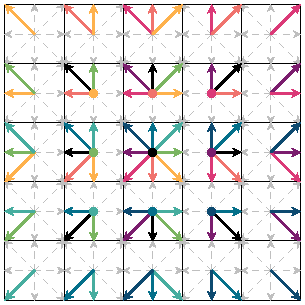
\includegraphics{streaming-after.pdf}
		\caption{After}
	\end{subfigure}
	\caption{Fluid vectors before and after the streaming step highlighted in color. Gray vectors are not considered.}
	\label{fig:streaming-step}
\end{figure}

\subsection{Boundary conditions}

There are two boundaries condition that needs to be implemented in this problem: wall and density. Since we want this to be a complete framework for two-dimensional fluid simulation, we also implemented the density boundary condition for completeness' sake.

\paragraph{Directional density boundary condition} This boundary condition can be achieved by explicitly setting the value of $f_0$ to $f_8$ after a complete simulation step.

\paragraph{Wall boundary condition} This boundary condition is sometimes referred off as the bounce-back boundary condition. If the fluid from an adjacent cell is streamed into a wall located at $(n, m)$, the wall simply reflects the fluid vector back:
\begin{equation}
	f_j\ab(n - (\vv{e}_i \vdot \yhat), m - (\vv{e}_i \vdot \xhat)) = f_i(n, m) \label{eq:wall-boundary-calculation}
\end{equation}
where
\begin{equation}
	j = \begin{cases}
		i + 2 & \textrm{if} ~ i = 1, 2, 5, 6, \\
		i - 2 & \textrm{if} ~ i = 3, 4, 7, 8.
	\end{cases} \label{eq:wall-boundary-calculation-relation}
\end{equation}
Since the fluid cannot possibly stream into the center of the wall, $j$ doesn't have to be defined at $i = 0$. \cite{adams-no-date}

\paragraph{Wall-velocity boundary condition} Given a wall that's located at position $(n, m)$, and an exposed fluid cell located at position $\ab(n + (\vv{e}_a\vdot\yhat), m + (\vv{e}_b\vdot\xhat))$, the velocity boundary condition can be defined by two variables: velocity along $\vv{e}_a$, and along its clockwise perpendicular, $\vv{e}_b$ where
\begin{equation}
	b = \begin{cases}
		a + 3 & \textrm{if} ~ a = 1,       \\
		a - 1 & \textrm{if} ~ a + 2, 3, 4.
	\end{cases}
\end{equation}
Here, we define the other directions that are relative to direction $a$:
\begin{gather}
	\alpha = \begin{cases}
		a + 2 & \textrm{if} ~ a = 1, 2, \\
		a - 2 & \textrm{if} ~ a = 3, 4,
	\end{cases} \\
	\beta = \begin{cases}
		a + 1 & \textrm{if} ~ a = 1, 2, 3, \\
		a - 3 & \textrm{if} ~ a = 4,
	\end{cases} \\
	A = \begin{cases}
		a + 7 & \textrm{if} ~ a = 1,       \\
		a + 3 & \textrm{if} ~ a = 2, 3, 4,
	\end{cases} \\
	B = \begin{cases}
		a + 6 & \textrm{if} ~ a = 1, 2, \\
		a + 2 & \textrm{if} ~ a = 3, 4,
	\end{cases} \\
	C = \begin{cases}
		a + 5 & \textrm{if} ~ a = 1, 2, 3, \\
		a - 1 & \textrm{if} ~ a = 4,
	\end{cases} \\
	D = a + 4.
\end{gather}
These directions live on a grid relative to direction $a$ as illustrated in \cref{fig:relative-direction}.
\begin{figure}[ht]
	\centering
	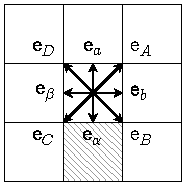
\includegraphics{relative-direction.pdf}
	\caption{Directions relative to the convention given by the wall-velocity boundary condition. The shaded region is the wall, and the cell with vector arrows is the target cell in which wall-velocity boundary condition is applied.}
	\label{fig:relative-direction}
\end{figure}
\begin{table}[ht]
	\centering
	\begin{tabular}{C C | C C C C C C}
		a & b & \alpha & \beta & A & B & C & D \\
		\hline
		1 & 4 & 3      & 2     & 8 & 7 & 6 & 5 \\
		2 & 1 & 4      & 3     & 5 & 8 & 7 & 6 \\
		3 & 2 & 1      & 4     & 6 & 5 & 8 & 7 \\
		4 & 3 & 2      & 1     & 7 & 6 & 5 & 8
	\end{tabular}
	\caption{Directions relative to the convention given by the wall-velocity boundary condition.}
	\label{tab:relative-direction}
\end{table}

Given that
\begin{equation}
	\vv{u}_a\ab(n + (\vv{e}_a\vdot\yhat), m + (\vv{e}_b\vdot\xhat)) \mathand \vv{u}_b\ab(n + (\vv{e}_a\vdot\yhat), m + (\vv{e}_b\vdot\xhat))
\end{equation}
is fixed by the boundary condition, the surrounding velocities in the cell $\ab(n + (\vv{e}_a\vdot\yhat), m + (\vv{e}_b\vdot\xhat))$ can be updated as follows: \cite{zou-1997}
\begin{gather}
	\vv{f}_a = \vv{f}_{\alpha} + \frac{2}{3}\rho\ab(n + (\vv{e}_a\vdot\yhat), m + (\vv{e}_b\vdot\xhat))\vv{f}_a, \label{eq:velocity-boundary-1} \\
	\vv{f}_A = \vv{f}_{C} - \frac{1}{2}\ab(\vv{f}_b - \vv{f}_{\beta}) + \rho\ab(n + (\vv{e}_a\vdot\yhat), m + (\vv{e}_b\vdot\xhat))\ab(\frac{\vv{u}_b}{6} + \frac{\vv{u}_a}{6}), \label{eq:velocity-boundary-2}\\
	\vv{f}_D = \vv{f}_{B} - \frac{1}{2}\ab(\vv{f}_b - \vv{f}_{\beta}) + \rho\ab(n + (\vv{e}_a\vdot\yhat), m + (\vv{e}_b\vdot\xhat))\ab(- \frac{\vv{u}_b}{6} + \frac{\vv{u}_a}{6}). \label{eq:velocity-boundary-3}
\end{gather}
For the rest of the directions, use the wall boundary condition (bounce-back) to calculate the fluids vector.

\chapter{Building the simulation framework}
\label{sec:model-building}

The implementation of the model in \texttt{Python} is different from the theoretical model due to some \texttt{NumPy} functions. This chapter serves as an overview for self-implementing the model. The codes in this chapter are not the actual code used in the \texttt{GitHub} repository. It's liberated from the object-oriented paradigms for ease of understanding. All of these will be pieced together in \cref{sec:model-structure}

This idea of implementing the simulation is actually an amalgamation of various ones. The article by \Citeauthor{adams-no-date} \cite{adams-no-date} and \Citeauthor{schroeder-2012} \cite{schroeder-2012} gave us a very comprehensive overview of the Lattice-Boltzmann method with boundaries condition, and also provided us with the intuition for creating our own ways of implementing. The inspiration for using the roll function is from \Citeauthor{matias-2022}'s video on Lattice-Boltzmann simulator \cite{matias-2022}. However, that video is quite old and uses a rather strange technique of implementing the boundary conditions, which leads to many numerical instabilities. Most of the time that's spent on this project is to make the boundary condition work. At the end, it did work, with the by product of sweat and tears. We don't want anyone to suffer through them with us. So, here is how we did it.

\section{Preliminary quantities}

The packages that are used throughout the project is imported as follows:
\begin{minted}{python}
import numpy as np
import matplotlib.pyplot as plt
import itertools as itr
from scipy.ndimage import convolve
import copy
import random
import math
\end{minted}
And, some useful arrays that are used throughout the project:
\begin{minted}{python}
unitVect = np.array(
    [[0, 0], [1, 0], [0, 1], [-1, 0], [0, -1], [1, 1], [-1, 1], [-1, -1], [1, -1]]
)
unitX = np.array([0, 1, 0, -1, 0, 1, -1, -1, 1])
unitY = np.array([0, 0, 1, 0, -1, 1, 1, -1, -1])
weight = np.array([4/9, 1/9, 1/9, 1/9, 1/9, 1/36, 1/36, 1/36, 1/36])
\end{minted}
The \texttt{unitVect} array represents the vector $\vv{e}_0,\dots,\vv{e}_8$. \texttt{unitX} and \texttt{unitY} array represents the dot product of these vectors to $\xhat$ and $\yhat$ respectively. Lastly, the \texttt{weight} array represents the weight that's used to calculate.

\section{Preliminary functions}

\subsection{Representation of physical quantities}

The whole lattice is represented as a \texttt{NumPy} array with dimensions $(N, M, 9)$. The first axis represents the $y$ index, second represents the $x$ index, and the third one with nine elements represent the fluid vectors $\vv{f}_0, \dots, \vv{f}_8$. Since these fluid vectors actually represents the amount of fluid that's travelling inside a cell, the vectors cannot be zero. Thus, the array is set to be all ones even when the fluid at rest. One can simply initialize the array as follows:
\begin{minted}{python}
yResolution = 24 # Configurable
xResolution = 36 # Configurable
fluid = np.ones(yResolution, xResolution, 9)
# The fluid array is to be modified according to the desired initial condition
initCondition = np.copy(fluid)
\end{minted}
The array \texttt{initCondition} serves as a reference for future plotting.

For simplicity, we also define two arrays that are used throughout: \texttt{yIndex} and \texttt{xIndex} which is an array filled with numbers from $0$ to $y - 1$, and $0$ to $x - 1$ respectively.
\begin{minted}{python}
yIndex = np.arange(yResolution)
xIndex = np.arange(xResolution)
\end{minted}

In the simulation step that is documented later in \cref{sec:simulation-function}, there must be a function that updates the density, momentum density, and velocity density of the fluid every time the simulation runs. First, we initialize the arrays that contain the density, momentum density, and the velocity density of the fluid according to \cref{eq:density-calculation,eq:momentum-calculation,eq:velocity-calculation}:
\begin{minted}{python}
density = np.sum(fluid, axis=2)
momentumY = np.sum(fluid * unitY, axis=2)
momentumX = np.sum(fluid * unitX, axis=2)
speedY = momentumY / density
speedX = momentumX / density
speedY = np.nan_to_num(speedY, posinf=0, neginf=0, nan=0)
speedX = np.nan_to_num(speedX, posinf=0, neginf=0, nan=0)
\end{minted}
These arrays are then updated using the following functions:
\begin{minted}{python}
def updateDensity():
    density = np.sum(fluid, axis=2)

def updateMomentum():
    momentumY = np.sum(fluid * unitY, axis=2)
    momentumX = np.sum(fluid * unitX, axis=2)

def updateSpeed():
    updateDensity()
    updateMomentum()

    speedY = momentumY / density
    speedX = momentumX / density
    speedY = np.nan_to_num(speedY, posinf=0, neginf=0, nan=0)
    speedX = np.nan_to_num(speedX, posinf=0, neginf=0, nan=0)
\end{minted}
Since \texttt{updateSpeed} calls both \texttt{updateDensity} and \texttt{updateMomentum}, one doesn't have to call \texttt{updateDensity} and \texttt{updateMomentum} when the function \texttt{updateSpeed} is already called.

\subsection{Wall boundary conditions}

The wall boundaries condition is stored as another array with dimensions $(N, M)$ filled with boolean elements. If a position $(n, m)$ is \texttt{True}, then it is not a wall, else, it's a wall. This array can be used to easily impose the wall boundary condition on the \texttt{fluid} array. I.e., every point where there's a wall, there must be zero fluid; thus, the fluid vectors at those points shall be zero.
\begin{minted}{python}
boundary = np.full((yResolution, xResolution)) # Can be edited to be any shape desired.
fluid[boundary, :] = 0
\end{minted}

There are two types of wall that's implemented in this framework: circular, border, and rectangular; with their own functions. The cylindrical wall function takes in the boundary array that's to be modified (\texttt{boundary}), the cylinder's center (\texttt{cylinderCenter}) as a tuple in the format $(y, x)$, and the cylinder's radius (\texttt{cylinderRadius: float}) as a floating point number:
\begin{minted}{python}
def cylindricalWall(boundary, cylinderCenter: tuple, cylinderRadius: float):
    for yIndex, xIndex in itr.product(
        range(yResolution), range(xResolution)
    ):
        if math.dist(cylinderCenter, [yIndex, xIndex]) <= cylinderRadius:
            boundary[yIndex, xIndex] = True
\end{minted}
The border wall function takes in the boundary array (\texttt{boundary}), and the thickness of the border (\texttt{thickness: int = 1}) as an integer:
\begin{minted}{python}
def borderWall(boundary, thickness: int = 1):
    boundary[0 : yResolution, -1 + thickness] = True
    boundary[0 : yResolution, xResolution - thickness] = True
    boundary[-1 + thickness, 0 : xResolution] = True
    boundary[yResolution - thickness, 0 : xResolution] = True
\end{minted}
The rectangular wall function takes in the boundary array (\texttt{boundary}) and the position of the two corner points (\texttt{cornerCoord1: tuple, cornerCoord2: tuple}) as a tuple in the format $(y, x)$.
\begin{minted}{python}
def filledStraightRectangularWall(
    boundary,
    cornerCoord1: tuple,
    cornerCoord2: tuple
):
    maxY = max(cornerCoord1[0], cornerCoord2[0])
    minY = min(cornerCoord1[0], cornerCoord2[0])
    maxX = max(cornerCoord1[1], cornerCoord2[1])
    minX = min(cornerCoord1[1], cornerCoord2[1])

    for yIndex, xIndex in itr.product(
        range(yResolution), range(yResolution)
    ):
        if (
            (xIndex <= maxX)
            and (xIndex >= minX)
            and (yIndex <= maxY)
            and (yIndex >= minY)
        ):
            boundary[yIndex, xIndex] = True
\end{minted}
These functions directly modifies the \texttt{boundary} array. They must be called before imposing the wall boundaries to the \texttt{fluid} array.

In some cases, it's more desirable to use the indices of the boundaries instead. We also write another function that's used to generate the indices of the boundaries. This function takes in the boundary array (\texttt{boundary}), and outputs two arrays: \texttt{boundaryIndex}, which is a list containing the indices of walls, and \texttt{invertedBoundaryIndex}, which is a list that contains the indices of fluids (invert of walls).
\begin{minted}{python}
def generateIndex(boundary):
    boundaryIndex = []
    invertedBoundaryIndex = []
    for i, j in itr.product(
        range(yResolution), range(xResolution)
    ):
        if boundary[i, j] != False:
            boundaryIndex.append((i, j))
        else:
            invertedBoundaryIndex.append((i, j))
    return boundaryIndex, invertedBoundaryIndex
\end{minted}

Since the end goal of this project is to simulate air conditioner placements, we also have to know the possible indices that the air conditioner can end up at. Therefore, we build a function \texttt{generateACPos} that can do so:
\begin{minted}{python}
def generateACDirections(boundary):
    possibleACPos = []
    for shiftIndex, axisIndex in itr.product([-1, 1], [1, 0]):
        shiftedBoundary = np.roll(boundary, shift=shiftIndex, axis=axisIndex)
        possibleACPos = np.logical_or(
            possibleACPos,
            np.logical_not(boundary) & shiftedBoundary
        )
    return possibleACPos
\end{minted}
This function takes in a boundary (\texttt{boundary}), then return a list of possible air conditioner positions (\texttt{possibleACPos}). It works by shifting the array \texttt{boundary} in the four cardinal directions ($i = 1, 2, 3, 4$) using the \texttt{np.roll} function, then comparing the shifted array to the original array. If a point $(n, m)$ in the original array isn't a wall, but the point $(n, m)$ on the shifted array along direction $i$ isn't a wall, then the point $(n, m)$ can hold an air conditioner that faces the direction $i$. All the possible points from all the shifted directions are combined using an or gate to obtain an array that contains all the point that can hold an air conditioner (\texttt{possibleACPos}).

The last function of the wall boundary condition is a function that turns the two-dimensional contour of the possible air conditioner position into a single continuous line called \texttt{indexPossibleACPos}. This has to be done because the gradient descent algorithm that is used to find the optimal air conditioner placement has to take in a continuous variable as its parameters. This can be done by a breadth first search along the line.
\begin{minted}{python}
def indexPossibleACPos(possibleACPos, clear: bool = False):
    testArray = copy.deepcopy(possibleACPos)
    currentIndex = tuple()
    for yIndex, xIndex in itr.product(
        range(yResolution), range(xResolution)
    ):
        if testArray[yIndex, xIndex]:
            currentIndex = (yIndex, xIndex)
            break

    while testArray[currentIndex]:
        for latticeIndex in [1, 2, 3, 4, 5, 6, 7, 8, 0]:
            nextIndex = addTuple(
                currentIndex,
                (
                    unitX[latticeIndex],
                    unitY[latticeIndex],
                ),
            )
            if testArray[nextIndex]:
                possibleACIndex.append(nextIndex)
                testArray[currentIndex] = 0
                currentIndex = nextIndex
                break
            else:
                pass
\end{minted}

\subsection{Density boundary condition} This is the easiest boundary condition to impose. One can just set the fluid vectors directly. Although I want this chapter to be liberated from object-oriented programming paradigm, this one just can't. Therefore, I shall introduce a new simple class: the \texttt{DensityBoundary} class:
\begin{minted}{python}
class DensityBoundary:
    def __init__(self, y: int, x: int, magnitude: float, direction: int):
        self.y = y
        self.x = x
        self.magnitude = magnitude
        self.direction = direction
\end{minted}
This class contains the position of the density boundary condition (\texttt{y} and \texttt{x}), the magnitude of density, and the direction that the density is imposed. The density boundary condition is imposed as follows:
\begin{minted}{python}
velocityBoundaries = []
def imposeDensityBoundaryCondition(boundary, velocityBoundaries):
    for velocityBoundary in velocityBoundaries:
        fluid[
            velocityBoundary.y, velocityBoundary.x, velocityBoundary.direction
        ] = velocityBoundary.magnitude
    updateSpeed()
\end{minted}

\subsection{Wall-velocity boundary condition}

The wall-velocity boundary condition is also implemented as a class which is initialized with the $(y, x)$ position of the boundary condition and the velocity along direction $\vv{e}_a, \vv{e}_b$.
\begin{minted}{python}
class VelocityBoundary:
    indices = [[1, 8, 5], [2, 5, 6], [3, 6, 7], [4, 7, 8]]

    def __init__(self, y: int, x: int, ux, uy, direction: int):
        self.y = y
        self.x = x
        self.uy = uy
        self.ux = ux
        self.direction = direction

        # For calculating the ua and ub
        if direction in [3, 4]:
            reflectIndex = direction - 2
        else:
            reflectIndex = direction + 2

        self.mainVelocity = ux if direction in [1, 3] else uy
        self.minorVelocity = uy if direction in [1, 3] else ux
        self.setIndices = VelocityBoundary.indices[direction - 1]
        self.getIndices = VelocityBoundary.indices[reflectIndex - 1]
\end{minted}
All the pressure boundaries point are then stored as an object of the class \texttt{VelocityBoundaries} in a list called \texttt{velocityBoundaries}. We then iterate over the list to update the fluid simulation grid according to \cref{eq:velocity-boundary-1,eq:velocity-boundary-2,eq:velocity-boundary-3}.
\begin{minted}{python}
velocityBoundaries = [] # A list of pressure boundaries point
def imposeVelocityBoundaryCondition(fluid):
    for velocityBoundary in velocityBoundaries:
        for latticeIndex in range(9):
            fluid[velocityBoundary.y, pressureBoundary.x, latticeIndex] = 0
        densityAtIndex = density[velocityBoundary.y, pressureBoundary.x]
        fluid[
            velocityBoundary.y, pressureBoundary.x, pressureBoundary.setIndices[0]
        ] = fluid[
            velocityBoundary.y, pressureBoundary.x, pressureBoundary.getIndices[0]
        ] + (
            2 / 3
        ) * (
            velocityBoundary.mainVelocity
        )
        fluid[
            velocityBoundary.y, velocityBoundary.x, velocityBoundary.setIndices[1]
        ] = (
            fluid[
                velocityBoundary.y,
                velocityBoundary.x,
                velocityBoundary.getIndices[1],
            ]
            - (
                0.5
                * (
                    fluid[
                        velocityBoundary.y,
                        velocityBoundary.x,
                        (
                            4
                            if velocityBoundary.direction - 1 == 0
                            else velocityBoundary.direction - 1
                        ),
                    ]
                    - fluid[
                        velocityBoundary.y,
                        velocityBoundary.x,
                        (
                            1
                            if velocityBoundary.direction + 1 == 5
                            else velocityBoundary.direction + 1
                        ),
                    ]
                )
            )
            + (0.5 * densityAtIndex * velocityBoundary.minorVelocity)
            + (1 / 6 * densityAtIndex * velocityBoundary.mainVelocity)
        )
        fluid[
            velocityBoundary.y, velocityBoundary.x, velocityBoundary.setIndices[2]
        ] = (
            fluid[
                velocityBoundary.y,
                velocityBoundary.x,
                velocityBoundary.getIndices[2],
            ]
            + (
                0.5
                * (
                    self.fluid[
                        velocityBoundary.y,
                        velocityBoundary.x,
                        (
                            4
                            if velocityBoundary.direction - 1 == 0
                            else velocityBoundary.direction - 1
                        ),
                    ]
                    - self.fluid[
                        velocityBoundary.y,
                        velocityBoundary.x,
                        (
                            1
                            if velocityBoundary.direction + 1 == 5
                            else velocityBoundary.direction + 1
                        ),
                    ]
                )
            )
            - (0.5 * densityAtIndex * velocityBoundary.minorVelocity)
            + (1 / 6 * densityAtIndex * velocityBoundary.mainVelocity)
        )
\end{minted}

\section{Simulation functions}
\label{sec:simulation-function}

Here, it's time to write the actual code for simulating the fluid. There are three functions that are used: \texttt{streamFluid}, \texttt{bounceBackFluid}, and \texttt{collideFluid}. All of which follows the main steps of the Lattice-Boltzmann method: streaming, self-collision, and wall boundary.

\paragraph{Streaming step} Earlier, we calculated the value of $\vv{e}_i\vdot\yhat$ and $\vv{e}_i\vdot\xhat$, and stored it into the array \texttt{unitX} and \texttt{unitY}. These quantities are then used to shift the array in their respective directions, representing the streaming step.
\begin{minted}{python}
def streamFluid(fluid):
    for latticeIndex, shiftY, shiftX in zip(
        range(9), unitY, unitX
    ):
        fluid[:, :, latticeIndex] = np.roll(
            fluid[:, :, latticeIndex], shiftY, axis=0
        )
        fluid[:, :, latticeIndex] = np.roll(
            fluid[:, :, latticeIndex], shiftX, axis=1
        )
\end{minted}

\paragraph{Self-collision step} The code follows from \cref{eq:self-collision-calculation-1,eq:self-collision-calculation-2}. It iterates through every fluid vectors in a lattice and update them accordingly.
\begin{minted}{python}
def collideFluid(fluid):
    fluidEquilibrium = np.zeros(fluid.shape)
    for latticeIndex, cy, cx, w in zip(
        range(9), unitY, unitX, weight,
    ):
        fluidEquilibrium[:, :, latticeIndex] = (
            density
            * w
            * (
                1
                + 3 * (cx * speedX + cy * speedY)
                + 9 * (cx * speedX + cy * speedY) ** 2 / 2
                - 3 * (speedX**2 + speedY**2) / 2
            )
        )
    fluid += (fluidEquilibrium - fluid) / relaxationTime
\end{minted}

\paragraph{Imposing wall boundary condition} We define a dictionary \texttt{reflectIndices} to convert from the index that's pointing into the wall to the index that points opposing the wall. The elements of the dictionary directly reflect the relation given by \cref{eq:wall-boundary-calculation-relation}. The part that updates the fluid directly reflects \cref{eq:wall-boundary-calculation}.

\begin{minted}{python}
boundaryIndex, invertedBoundaryIndex = generateIndex(boundary)
reflectIndices = {0: 0, 1: 3, 2: 4, 3: 1, 4: 2, 5: 7, 6: 8, 7: 5, 8: 6}
def bounceBackFluid(fluid):
    for y, x in boundaryIndex:
        for latticeIndex in range(9):
            if fluid[y, x, latticeIndex] != 0:
                bounceIndexY = y - unitY[latticeIndex]
                bounceIndexX = x - unitX[latticeIndex]
                if (bounceIndexY >= 0 and bounceIndexY < yResolution) and (
                    bounceIndexX >= 0 and bounceIndexX < xResolution
                ):
                    fluid[
                        bounceIndexY,
                        bounceIndexX,
                        reflectIndices[latticeIndex],
                    ] = fluid[y, x, latticeIndex]
                    fluid[y, x, latticeIndex] = 0
    updateSpeed()
\end{minted}

\section{Main loop}

We first define a counter that counts the amount of times that we ran the simulation: \texttt{step}. For further comparison, we deep-copy the state of the fluid before updating to the variable \texttt{lastStepFluid}. Then, the fluid vector is updated in order: stream, bounce back, self-collide, impose velocity, and impose density.
\begin{minted}{python}
def stepSimulation(fluid):
    lastStepFluid = copy.deepcopy(fluid)
    streamFluid()
    bounceBackFluid()
    collideFluid()
    imposeVelocityBoundaryCondition()
    imposePressureBoundaryCondition()
    step += 1
\end{minted}

\chapter{Model structure}
\label{sec:model-structure}

\chapter{Optimization algorithm}

\section{Implementation}


\printbibliography

\end{document}
